 \documentclass[../IoMusT.tex]{subfiles}
\begin{document}
\subsection{Prezentarea scurtă a aplicației finale}
Cu ajutorul tehnologiilor software și hardware scopul acestei lucrări a fost de a crea un dispozitiv care va veni în ajutor în comunitatea surdă când vine vorba despre ascultarea muzicii la un instrument anume. Datorită faptului că celelalte simțuri a acestor persoane sunt mult mai dezvoltate am mers pe idea de a crea o aplicația care să redea nu numai vibrațiile muzicii ci și să facă și o reprezentare cât mai bună posibilă a acestor note în culori. Astfel utilizatorii vor putea avea și o experiență vizuală plăcută pe lângă cea tactilă. Pentru a face posibilă acest lucru mai întâi s-a dezvoltat o aplicație pe placa de dezvoltare Raspberry Pi, care are ca scop atât colectarea și trimiterea informațiilor de la pian câtre aplicația Android cât și redarea vibrațiilor cu ajutorul motoarelor LRA. Aplicația Android a venit ca o completare a acestui proiect din nevoia personalizării experienței a utilizatorilor și pentru redarea efectului vizual din datele primite de la placa de dezvoltare Raspberry Pi. În ambele părți s-au folosit tehnologii prezentate în capitolele anterioare iar în cele ce urmează se vor detalia atât metodele de implementare alese cât și cum s-a ajuns la varinata finală în ceea ce privește structura hardware a lucrării.
\subsection{Implementarea aplicației pe placa de dezvoltare RaspberryPi}
\subsubsection{Metode de asamblare a componentelor hardware}
%adaugare poze cu asamblarea	
Pentru realizarea dispozitivului purtabil s-a folosit nouă bucăți de motoare de tip LRA conectate da placa de dezvolatre Raspberry Pi. Datorită faptului că pentru acest număr de motoare trebuie 9 pini de ground, iar placa are numai 8 la bucăți, s-a folost un breadboard  pe care se poate conecta un singur pin de ground. Conectarea, după cum se vede și din figura ... s-a făcut cu ajutorul unor cabluri de tip tată-tată și mamă-tată, motoarele de vibrații fiind și ele lipite  de aceste fire pentru un contact mai bun.
\\
\par Numărul total de motoare de vibrații LRA folosite influențează experiența utilizatoruluil din motive destul de evidente. Mai multe motoare înseamnă vibrații intensificate și de mai multe feluri. Datorită faptului că am folosit un instrument muzical cu o gamă largă de note era evident că pentru a avea un rezultat cât mai bun este nevoie de mai multe motoare. Nu s-au folosit un număr mai mare de motoare decât nouă din cazua posibilităților de echipamente hardware. Modul în care aceste motoare sunt distributie și vibrează este în felul următor: folosind un pian electric cu 61 de clape am împărțit aceste clape în trei categorii de note muzicale. Primele două octave (adică notele joase) reprezintă prima categorie. A doua categorie reprezintă notele din mijloc, aceasta fiind formată numai dintr-o ocatvă. Ultima categorie este reprezentată de cele două octave rămase adică notele cele mai înalte. Fiecare astfel de categorie "primește"  trei motoare. Când se va apăsa o clapă una dintre cele trei categorii de motoare vor începe să vibreze la o anumită valoare și frecvență calculată. Metoda prin care au fost calculate aceste categorii se poate observa în figura \ref{fig:range} unde se verifică numărul MIDI a notei muzicale iar în funcție de asta se va returna un bulean.
\begin{figure}[h]
\centering
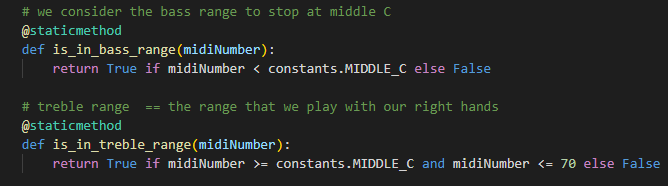
\includegraphics[scale=0.75]{range}
\caption{Împărțirea motoarelor în categorii}
\label{fig:range}
\end{figure}  
\\
\par Breadbourd-ul folosit pentru prototipare este unul cu 830 de puncte, având destul loc pentru conectarea motoarelor. Pentru conecatrea la ground s-a folosit un singur pin de pe placa de dezvoltare  Raspberry Pi, acesta fiind conectat la rândul corespunzător de pe breabdoard. Cei nouă pini folosiți pentru alimentarea cu tensiune sunt: 14, 15 și 18 pentru prima categorie, 17, 27, 22 pentru a doua respectiv 10, 9 și 11 pentru ultima categorie de motoare, fiecare dintre aceștia putând fi programat pentru modularea lățimii pulsului.
\\
\\
- secțiunea aceasta va mai fi completată cu poze cu dispozitivul asamblat (firele sunt lipite, trebuie doar să le conectez într-un mod corespunzător la breadboard)
\subsubsection{Metoda de calculare folosită pentru motoarele de vibrații}
Calcularea intensității și a frecvenței cu care vibrează un motor se face pe baza notei MIDI primite de la pian. Nota muzicală cântată ajunge sub forma unui număr în programul nostru asta însemnând că cu cât e mai mare numărul respectiv cu atât nota muzicală cântată este mai înaltă. Pentru că există formulă numai pentru calcularea frecvenței, pentru calcularea valorii am mers mai insinctiv.
\\
\par Știm că un motor de vibrații în cazul nostru poate lua valori între 0 și 1, asta însemnând că cu valoarea 0.5 motorul ar avea o vibrație decentă, fără prea multă putere. Luând această valoarea ca baza, am folosit regula de trei simpli pentru a calcula valoarea notei cântate. Nota care va vibra cu valoarea 0.5 am ales să fie A4 (la) fiind referința de ton care sunt reglate celelalte instrumente muzicale, acesta având și o frecvență întreagă (440 Hz) și fiind și clapa care este aprope de mijlocul pianului. O parte a metodei în care se calculează aceste valori se poate vedea în figura \ref{fig:calculateValue}.
\begin{figure}[h]
\centering
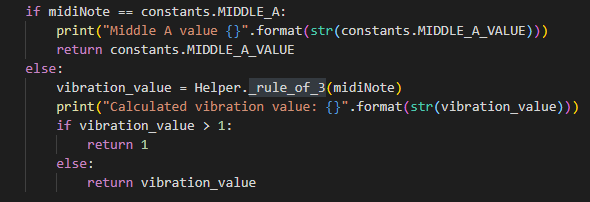
\includegraphics[scale=0.9]{calculateValue}
\caption{Calcularea valorii unei vibrații}
\label{fig:calculateValue}
\end{figure}  
 Știind că nota la este baza după care se calculează celelate note, apăsarea acestuia nu va chema metoda ce returnează rezultatele de la regula de 3 simpli. În cazul în care valoarea calculată este mai mare decât 1, se va returna valoarea 1 datorită faptului că biblioteca Mido va arunca excepție în caz contrar. Pentru valori mai mici de 0 nu o să avem caz pentru că este imposibil să primim un număr negativ. Metoda care calculează regula de trei simpli este prezentată în figura \ref{fig:ruleOf3}, unde \verb|MIDDLE_A| reprezintă numărul MIDI a notei muzicale A4 iar (69) iar \verb|MIDDLE_A_VALUE| este valoarea 0.5. Cu această metodă vom avea o distribuire în ceea ce privește aceste valori. Notele joase vor fi simțite cu o intensitate mai mare în timp ce notele mai înalte se vor simți mai puțin (în acest caz valoarea nu scade prea mult, va fi în jurul valorii 0.2, ceea ce încă se poate simți).
\begin{figure}[h]
\centering
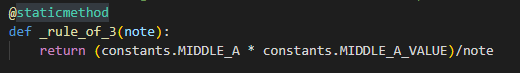
\includegraphics{ruleOf3}
\caption{Regula de 3 simpli}
\label{fig:ruleOf3}
\end{figure}  
\\
\par Formula cu care se calculează frecvența notelor muzicale a fost deja descris în subcapitolul 3.3. Utilizarea acestor valori (înafară setarea vibrației) se va discuta în subcapitolul ce urmează, acesta fiind folosit și în aplicația Android.
\subsubsection{Implementarea firelor de execuție pentru evitarea blocajului}
- descriere de ce este nevioe in acest caz sa folosim fire de executie
\\
\\
- descrierea modului de implementare a acestor fire de executie
\subsubsection{Comunicarea dintre firele de execuție} % aici despre cozi si evenimente
Datorită faptului că această aplicație se rulează pe mai multe fire de execuție este important să avem o comunicare bine sincronizată dintre aceastea în momentul cănd dorim să schimbăm mesaje între ei. Utilizarea socket-urilor impune folosirea unui fire de execuție separat ceea ce înseamnă că în momentul trimiterii sau a primii unor date, trebuie să avem acces la o memorie comună la care au acces ambele fire de execuție pentru a putea face schimb de informații. În cazul acestei aplicații trimiterea acestor datelor se face de pe ambele părți: atât aplicația Android cât și cea de pe placa de dezvoltare trebuie să trimită și să primească informații, ce vor fi parsate în următoarele etape.
\\
\par Gestionarea memoriei comune în aplicația de pe placa de dezvoltare se întâmplă cu ajutorul unei cozi. În momentul în care se primesc date, acestea sun decodate și puse în coadă. Celalalt fir de execuție, care trebuie să parseze aceste mesaje, preia informațiile din ea. Coada nu râmăne niciodată plină, mereu se scoate toată informația din ea de către celălalt fir de execuție. Pentru a putea implementa aceste acțiuni avem nevoie să știm momentul în care putem prelua aceste informații din coadă, din moment ce acestea nu vin încontinuu.
\\
\par Evenimentele din biblioteca \verb|threading| ne vin în ajutor în momentul în care dorim să primim o notificare că s-a întâmplat un lucru, fiind cel mai simplu mod de a comunica unui al fir de execuție că a avur loc a acțiune. Acestea funcționează ca niște booleane care pot fi setate în momentul în care s-a întâmplat o acțiune. În cazul nostru de fiecare date cănd se pune sau se ia un element în coadă, acest eveniment este setat pe \verb|True| respectiv pe \verb|False|  (a se vedea figura \ref{fig:ev}). Verificarea stării acestui eveniment se face prin apelarea metodei \verb|is_set()|.
\begin{figure}[h]
\centering
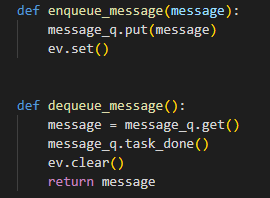
\includegraphics[]{ev}
\caption{Setare eveniment}
\label{fig:ev}
\end{figure}  
Setarea evenimentului se verficiă în momemntul în care citim datele de la pian. Datorită faptului că mesajele ce vin de pe aplicația Android influențează modul în care motoarele vor vibra, trebuie să preluăm și să parsăm aceste mesaje înaintea să setâm valoarea și frecvența motoarelor. În momentul în care acest eveniment a fost setat pe \verb|True|, se apelează o metoda din figura \ref{fig:processEv} care va procesa aceste date iar în funție de rezultate se vor modifica niște valori dintr-un dicționar. Mesajele primite vor fi mereu compuse din două cuvinte, deci parsarea lor este una ușoară. După ce mesajul a fost scos din coadă, evenimentul va fi setat pe \verb|False| până când un nou mesaj va fi introdus.
\begin{figure}[h]
\centering
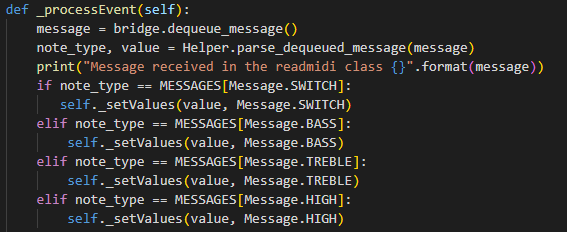
\includegraphics[scale=0.85]{processEv}
\caption{Parsare mesaje}
\label{fig:processEv}
\end{figure}  
\subsection{Integrarea unei aplicații mobile în proiect}
\subsubsection{Nevoia de folosire a unui aplicații Android}
Aplicația de placa de dezvoltare Raspberry Pi, după cum s-a discutat și în capitolele anterioare, oferă posibilitatea redării muzicii cântate la pian în formă de vibrații. Utilizatorul acestui dispozitiv, fără o aplicație conectată, nu are nici un fel de control asupra acestor lucruri, nu poate să intervină să oprescă sau să personalizeze vibrațiile simțite. Crearea unei aplicații Android pentru acest dispozitiv nu are scopul doar de a controla aceste vibrații dar și de a oferi un feedback vizual în ceea ce privește aceste note muzicale. 
\\
\par În subcapitolele ce urmează vor fi prezentați atât funcționalitățile incluse în aplicația Android cât și algoritmii aleși pentru implementarea acestora.
\subsubsection{Prezentarea UI-ului aplicației mobile}
Interfața aplicației mobile a fost făcut în așa fel încă să fie cât mai ușor de utilizat.
\subsubsection{Metoda de calcul pentru modificarea intensităților motoarelor de vibrații}
Modificarea intensităților cu care motoarele conectate vibrează este o funcționalitatea a cărui implementare necesită recalcularea valorilor cu ajutorul niștor formule. Am încercat să aleg metoda cea ma corectă de a calcula aceste schimbări astfel încât rezultatul final să fie unul cât mai corect și mai vizibil. Pe partea de aplicație Android am implementat numai partea de interfață a acestei funcționalități, urmând ca în aplicația de pe placa de dezvoltare Raspberry Pi să se facă calculelel necesare.
\\ %limita
\par În aplicația Android schimbarea valorilor a fost implementată cu ajutorul unei bare de progres. Aceste bare, a căror progrese pot fi setat manual de către utilizator, pot lua valori întregi într-o anumită limită ce poate fi specificată în cod. În cazul nostru aceste valori sunt cuprinse între 0 și 100, valoarea implicită fiind 50 datorită faptului că intensitatea poate să și scadă, nu numai să crească. Astfel dacă un utilizator trage bara de progres până la valoarea 0, intensitatea va scădea iar la 100 va crește cu până la 0.3 de valori. În momentul în care aplicația a sesizat o schimbare de valori în bara de progres, se trimite valoarea curentâ prin socket câtre aplicația de pe placa de dezvoltare. Mesajul se trimite sub forma unor două cuvinte (a se vedea figura \ref{fig:sendProgress}), toate mesajele fiind trimise așa pentru o parsare mai ușoară. Astfel în aplicația scrisă în python, prin despărțirea acestor două cuvinte, putem să ne dăm seama ușor operațiile ce trebuie făcute după primirea mesajelor.
\begin{figure}[h]
\centering
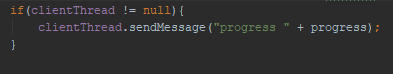
\includegraphics[]{sendProgress}
\caption{Trimiterea valorii barei de progres}
\label{fig:sendProgress}
\end{figure} 
\\
\par Calculul pentru schimbarea valorii a fost gândită în felul următor: dacă utilizatorul schimbă bara de progress cu 10 valori (de la 50 la 60 sau de la 50 la 40), intensitatea motoarelor se va ridica sau va scădea cu același procent. Așa pentru o schimbare de 50 de valori (de la 50 la 100 sau de la 50 la 0) va produce în ambele cazuri o recalculare a valorilor de vibrații de 0.3. În aplicația python, cu ajutorul unui dicționar este păstrat valoarea implicită a acestui porgres (50), astfel modificările de valori se vor întâmpla doar în cazul în care acest progres este diferit de valoarea implicită (a se vedea figura \ref{fig:not50}). În această situație este calculat o valoarea adițională care va fi adăugat la valoarea calculată în mod normal.
\begin{figure}[h]
\centering
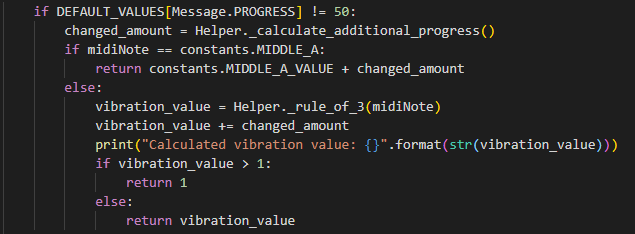
\includegraphics[scale=0.8]{progressNot50}
\caption{Calculul valorii cu pogres schimbat}
\label{fig:not50}
\end{figure} 
\\
\par Metoda care calculează valarea adițională care va fi adăugată are la bază o regulă de trei simpli. Se verifică dacă valoarea progresului trimis de pe aplicația Android este mai mic sau mai mare decât 50 pentru a ști dacă noua valoarea returnată trebuie sau nu să fie un număr negativ. Pentru că știm că valoarea maximă cu care se poate schimba bara de progres este de 50 și în cazul acesta intensitatea se schimbă cu 0.3, este ușor de calculat cu cât se schimbă intensitatea motoarelor de vibrații dacă valoarea acestui bare este diferit de 50. Acest calcul se poate observa în figura \ref{fig:additionalProgress}, unde \verb|MAX_MIN_PROGRESS_VALUE| este valoarea cu cares se poate schimba intensitatea motoarelor de vibrații iar \verb|DEFAULT_VALUE_FOR_SLIDER| este valoarea implicită pe care o are bara și totodată valoarea maximă cu care se poate schimbă ce implicită.
\begin{figure}[h]
\centering
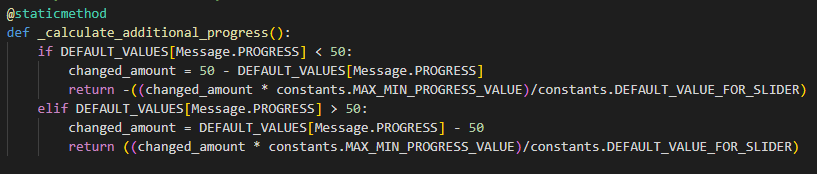
\includegraphics[scale=0.6]{additionalProgress}
\caption{Progress adițional}
\label{fig:additionalProgress}
\end{figure} 
\subsubsection{Realizarea comunicarii cu aplicația RaspberryPi}
- conectarea cu sockets
\\
\\
-descriere metode de decodare a datelor ajunse pe aplicatia android
\subsubsection{Integrarea vizualizării culorilor cu ajutorul frecvențelor}
-descriere metode alese pentru afisarea culorii in Android studio
\\
\\
- explicarea necesitatii frecventelor pentru a realiza acest lucru
\\
\\
- exemplificare cu cod cum s-au calculat reprezentarile hexa
\\
\\
-functionalitatea aceasta este inca in curs de implementare
\subsubsection{Prezentarea bazei de date folosite în aplicația Android}
\end{document}